\documentclass[11pt,a4paper,twoside,titlepage,BCOR12mm,DIV12]{scrartcl}
\usepackage{helvet}     % font 
\typearea[current]{last} % recalculate div for font

\usepackage{ngerman}    % german
\usepackage[latin1]{inputenc} %encoding
%\usepackage[T1]{fontenc}
%\usepackage{ae}

%distinction between latex and pdftex
\usepackage[pdftex]{graphics}   % pictures
%\usepackage{graphics}  % pictures

\usepackage{fancyhdr}   % page headers and footers
\usepackage{ifthen}     % used for changing appendix name layout
\usepackage{textcomp}   % special signs
\usepackage{url}        % as the name suggests
\usepackage{listings}   % program listings
\usepackage{tabularx}   % other tables


\def\myTitle{Entwicklung eines Bootloader f�r �ber CAN verbundene Mikrocontroller}
\def\myAuthorFirst{J�rg}
\def\myAuthorFamily{Diederich}

\newif\ifpdf
\ifx\pdfoutput\undedined
  \pdffalse
\else
  \pdfoutput=1
  \pdftrue
\fi

%distinction between latex and pdftex
\ifpdf
\usepackage[pdftex, pdfcreator=pdflatex]{hyperref}   % pdf internal links
\else
\usepackage[dvips,pdfcreator={dvipdf with dvips and ESP Ghostscript 7.07}]{hyperref}   % pdf internal links
\fi

% set overall font
\renewcommand{\familydefault}{\sfdefault}

% fancy headers
\fancyfoot{}
\fancyhead{}
\fancyhead[ER]{\nouppercase{\leftmark}}
\fancyhead[OL]{\nouppercase{\rightmark}}
\fancyhead[EL,OR]{\thepage}
\renewcommand{\sectionmark}[1]{%
        \markboth{\small \thesection{} #1}{\small \thesection{} #1}%
}
\renewcommand{\subsectionmark}[1]{%
        \markright{\small \thesubsection{} #1}%
}
\fancypagestyle{plain}{%
        \fancyfoot{}%
        \fancyhead[ER]{}%
        \fancyhead[OL]{}%
        \fancyhead[EL,OR]{}%
        \renewcommand{\headrulewidth}{0pt}%
        \renewcommand{\footrulewidth}{0pt}%
}
\fancypagestyle{appendix_deep}{%
  \fancyhead[ER]{\appendixname \, \nouppercase{\leftmark}}
  \fancyhead[OL]{\appendixname \, \nouppercase{\rightmark}}
}
\fancypagestyle{appendix_flat}{%
  \fancyhead[ER]{\appendixname \, \nouppercase{\leftmark}}
  \fancyhead[OL]{}
}
\fancypagestyle{reset}{%
  \fancyhead[ER]{\nouppercase{\leftmark}}
  \fancyhead[OL]{\nouppercase{\rightmark}}
  \fancyhead[EL,OR]{\thepage}
}
\pagestyle{fancy}

% indended list
\newenvironment{ilist}[1]
  {\begin{list}{}{%
   \settowidth{\labelwidth}{\textbf{#1}}%
   \setlength{\leftmargin}{\labelwidth}%
   \addtolength{\leftmargin}{\labelsep}%
   \renewcommand{\makelabel}[1]{\textbf{##1}\hfill}%
  }}
  {\end{list}} 

% new date: just month and year
\newcommand{\montoday}{\ifcase\month\or
 Januar\or Februar\or M\"arz\or April\or Mai\or Juni\or
 Juli\or August\or September\or Oktober\or November\or Dezember\fi
 \space\number\year} 

% different appendix layout, puts letter to the right
\newcommand*{\appendixmore}{%
  \DeclareRobustCommand*{\othersectionlevelsformat}[1]{
    \ifthenelse{\equal{##1}{section}}{%
      \appendixname~}{}%
    \csname the##1\endcsname\autodot\enskip}
  \renewcommand*{\sectionmarkformat}{%
    \appendixname~\thesection\autodot\enskip}
}

% roman enumerated list
\newenvironment{renumerate}{% defines new environment for list with roman labels
 \def\theenumi{(\roman{enumi})}%
 \renewcommand{\labelenumi}{(\roman{enumi})}%
 \begin{enumerate}}%
 {\end{enumerate}}

\makeatletter % necessary if in preamble, drop if in style file
\renewcommand{\@dotsep}{4.5} % defaults to 4.5
\makeatother % necessary if in preamble, drop if in style file 

% setup hyperref
\hypersetup{%
 setpagesize = false,
 pdftitle     = {\myTitle},
 pdfsubject = {Ausarbeitung zum Laborpraktikum},
 pdfauthor    = {\myAuthorFirst\ \myAuthorFamily},
 pdfkeywords = {Bootloader, CAN, AVR},
% pdfcreator = {pdflatex},
% pdfcreator = {dvipdf with dvips and ESP Ghostscript 7.07},
 pdfproducer = {LaTeX with hyperref},
 pdfview = Fit,
 pdfstartview = Fit,
 pdfpagelayout = SinglePage, % 'facing' does'nt exists :(
 pdfpagemode = UseOutlines,
 bookmarksnumbered = true,
 bookmarks = true,
 breaklinks = true,
 colorlinks = true, % no borders please, color the text instead
% non-printing environment
 linkcolor = blue
%
% printing environment
% linkcolor = black,
% citecolor = black,
% filecolor = black,
% urlcolor = black
}

% tabularx special columns
\newcolumntype{Y}{>{\centering\arraybackslash}X}%

% float handling
%   Parameters for TEXT pages (not float pages):
\setcounter{topnumber}{3}
\setcounter{bottomnumber}{3}
\setcounter{totalnumber}{6}     % 2 may work better



\begin{document}
% titlepage
\begin{titlepage}
\vspace*{\fill}
\begin{center}
{
  \Large 
  Otto-von-Guericke-Universit�t Magdeburg\\[5mm]

  \begin{figure}[htbp]
    \begin{center}
      \scalebox{0.15}{\rotatebox{0}{
\includegraphics{../pics/ovg}}}
    \end{center}
  \end{figure}

  Institut f�r Verteilte Systeme\\
  AG Eingebettete Systeme und Betriebssysteme\\[15mm]

  \huge\myTitle\\[10mm]

  \LARGE Laborpraktikumsbericht\\[20mm]

  \Large 
  \myAuthorFirst\/ \myAuthorFamily\\[3mm]
  \large Wintersemester 2006\\[10mm]

  \large Betreuer:\\[3mm]	
  \Large Prof. J�rg Kaiser\\
  \Large Dipl. Inform. Michael Schulze
}
\end{center}
\vspace*{\fill}
\end{titlepage}
\cleardoubleemptypage






%
% toc and preface
\pdfbookmark[1]{\contentsname}{tocanc}
\pagenumbering{Roman}
\tableofcontents
\cleardoublestandardpage

\listoffigures
\cleardoubleemptypage

\listoftables
\cleardoubleemptypage
%
%abstract
%\include{abstract}
%chapters
\pagenumbering{arabic}

%\section{Motivation und Aufgabenstellung}
%mehrere knoten. bisher jeder einzeln. das aufwendig. da sowieso verbunden, das
%ausnutzen.
\section{Motivation und Aufgabenstellung}
\label{l:motiv}
Die Softwareentwicklung f�r Mikrocontroller l�sst sich in zwei Phasen
unterteilen. In der ersten Phase, bis zum Abschluss der Implementierung, wird 
auf einem Fremdsystem entwickelt. Durch ihre weite 
Verbreitung kommen zumeist Personalcomputer zum Einsatz. 
Mit Verwendung von Crosscompilern l�sst sich Programmcode f�r den
gew�hlten Mikrocontroller erzeugen. Erst mit der �ber\-tragung des 
Programmcode 
auf den Mikrocontroller beginnt die zweite Phase der Softwareentwicklung, nun
auf dem beabsichtigtem Zielsystem.
\newline
Durch die F�higkeit von Mikrocontrollern zum sog. In-System-Programming
wird der �bergang zwischen beiden Entwicklungsphasen vereinfacht. Auf 
aufwendige 
Umbauma�nahmen der Hardware oder gar einem Ausbau des Mikrocontrollers aus 
einem kompletten System kann verzichtet werden. Vielmehr kann ein
Mikrocontroller, wie der Name schon vermuten l�sst, beim �bertragen von 
Programmcode im System verbleiben. Dies reduziert die mechanische 
Beanspruchung des gesamten Systems, zudem wird  
viel Zeit eingespart. Die gewonnene Flexibilit�t l�sst sich beispielsweise
f�r zus�tzliche Tests im Rahmen der Softwareentwicklung einsetzen.  
Das In-System-Programming ( im Folgendem auch kurz mit ISP bezeichnet) nutzt 
vorhandene Kommunikationsm�glichkeiten eines Mikrocontrollers. Bekannt sind 
serielle M�glichkeiten wie JTAG oder SPI. Ein entsprechendes Kabel samt
Adapter stellt dabei die Verbindung zwischen PC und 
Mikrocontroller her. 
\newline
Mikrocontroller der AT90CAN-Baureihe der Firma Atmel 
besitzen eine Schnittstelle f�r den CAN-Bus. Wird diese Schnittstelle als 
vornehmliche Kommunikationsm�glichkeit verwendet, erscheint die Verwendung 
einer zus�tzlichen Schnittstelle lediglich zum Zwecke des ISP �berfl�ssig.
\newline
Die M�glichkeit zum ISP �ber den existierenden CAN-Busanschluss bietet mehrere
Vorteile:
\begin{itemize}
        \item Es entf�llt das Anschlie�en eines 
        zus�tzlichen Verbindungskabels, wenn aus\-schlie�\-lich per CAN 
        kommuniziert wird. Zus�tzlich bleibt in diesem Falle eine 
        Schnittstelle des Mikrocontrollers st�ndig f�r andere Aufgaben frei.
        \item Es entf�llt der oft l�stige Wechsel des jeweils angeschlossenen 
        Mikrocontrollers. Bisherige Verfahren erlauben nur die Kommunikation 
        mit einem einzelnen Mikrocontroller. 
        F�r die Verwendung mehrerer Mikrocontroller muss bisher immer das 
        Verbindungskabel getrennt und neu angeschlossen werden. 
        \item Es wird zus�tzlich Zeit eingespart, da mehrere Mikrocontroller
        gleichzeitig mit neuem Programmcode versehen werden k�nnen.
        Gerade bei Verwendung mehrerer Mikrocontroller nimmt das bisher 
        praktizierte sequentielle Vorgehen viel Zeit in Anspruch.
        \item Letztendlich wird auch die mechanische Beanspruchung der 
        Anschl�sse reduziert. 
\end{itemize}
Ziel des durchgef�hrten Laborpraktikums war es, die genannten Vorteile durch
eine entsprechende Entwicklung nutzbar zu machen. Grundlage waren, wie bereits 
angedeutet, Mikrocontroller des Typs Atmel AT90CAN128. 
Die Aufgabe umfasste Konzeption eines Befehlprotokolls und 
entsprechende Programmierung der Mikrocontroller. Weiterhin galt es, einen 
entsprechenden Gegenpart auf Seite eines PC zu entwickeln. Als Resultat 
sollte der eingangs beschriebene Prozess der Softwareentwicklung f�r 
Mikrocontroller weiterhin durchf�hrbar sein.






%\section{Anforderungen}
%bootloader auf mcu-seite und client auf pc-seite.
%\subsection{Atmel AT90CAN Mikrocontroller}
%was kann der, was nicht.
%\subsection{Controller Area Network}
%feldbus. besonderheiten.
%\subsection{Programmiersoftware Avrdude}
%kurze erl�uterung, wie wird dort vorgegangen. was kann der. was nicht. 
%prog-sprache c. wie ablauf f�r benutzer.
\section{Anforderungen}
\label{l:anforderungen}
Die Anforderungen lassen sich in mehrere Bestandteile zerlegen. Zun�chst 
m�ssen die Eigenschaften der verwendeten Kommunikation beachtet werden. 
Weiterhin stellt der zu verwendende Mikrocontroller Anforderungen. 
Schlussendlich sind die Voraussetzungen zur Softwareentwicklung 
und die Anforderungen an die Funktionalit�t der L�sung zu ber�cksichtigen.

% standards. identifer, datenl�nge. arbitrierung.
\subsection{Controller Area Network CAN}
\label{l:can}
Der Begriff CAN bezeichnet einen seriellen Feldbus. F�r auf dem 
Bus versandte Nachrichten sind verschiedene Formate spezifiziert. F�r den 
unmittelbaren Datenaustausch interessant sind der sog. Daten-Frame und der 
Remote-Frame. Diese setzen sich im Wesentlichen aus folgenden Bestandteilen 
zusammen:
\begin{enumerate}
        \item Bezeichner (Identifier)
        \item Anzahl der Datenbytes (Data Length Code)
        \item Datenbytes (Data)
\end{enumerate}
\noindent Vervollst�ndigt wird die Nachricht durch verschiedene Bits und 
durch eine Checksumme. Andere spezifizierte Formate dienen der Steuerung des 
Datenflusses.
\newline
Die Kommunikation �ber CAN basiert nicht auf der Adressierung des Empf�ngers,
sondern auf der Kennzeichnung einer Nachricht \cite{etschberger}\/.
Die aktuelle CAN-Spezifikation CAN 2.0 sieht f�r den
Bezeichner einer Nachricht zwei verschiedene L�ngen vor. CAN 2.0A spezifiziert
einen sog. Standard-Identifier von 11 Bit L�nge. In CAN 2.0B wird der 
Identifier 
auf 29 Bit erweitert, in diesem Fall wird von einem Extended-Identifier 
gesprochen. �ber die Spezifikationen hinweg gleich bleibt die m�gliche 
Anzahl an Datenbytes: Nachrichten im CAN-Bus enthalten maximal 8 Byte 
Daten. Auch Nachrichten ohne Datenbytes sind zul�ssig. Die Anzahl enthaltener
Datenbytes wird durch das entsprechende Feld in einer Nachricht beschrieben.
\newline
Die CAN-Spezifikation ist unabh�ngig vom verwendeten �bertragungsmedium. 
Verf�g\-bar sind 
drahtgebundene und drahtlose bzw. optische L�sungen \cite{bosch}.
Aufgrund dieser Unabh�ngigkeit variiert der spezifizierte maximale Durchsatz.
In der gebr�uchlichen Spezifizierung nach {\it ISO 11898-2 high speed}\/,
welche die Verwendung von Twisted-Pair-Kabel vorsieht, sind maximal 
1 Mbit/s Durchsatz definiert.
\newline
Die Besonderheit des CAN-Busses ist die Arbitrierung nach CSMA/CA. Um 
Kollisionen im Falle eines gleichzeitigen Buszugriffs zu vermeiden, wird sich
des Bezeichners einer Nachricht bedient. Stellt ein Sender anhand des 
Bezeichners fest, dass seine Nachricht niedriger priorisiert ist als die 
Nachricht eines gleichzeitig sendenden anderen Teilnehmers, stellt er seinen 
Sendevorgang ein. Erst anschlie�end kann dieser Teilnehmer einen erneuten 
Sendeversuch durchf�hren. Auf diesem Wege wird der Buszugriff gesteuert 
und zudem der Versand der Nachricht mit dem h�chstpriorisiertem Bezeichner 
sichergestellt.
Im Falle des gleichzeitigen Versands von Nachrichten mit gleichen Bezeichnern
liegt ein Fehler vor. Dieser Zustand darf nicht eintreten, kann aber von den 
Teilnehmern erkannt und entsprechend behandelt werden.
 

% 8k boot flash, 4k ram. spm per irq. fuse-bits und boot-reset. irq-vector 
% move. programmierung per parallel, spi, jtag. 
% bootloader support 
% can-port nach 2.0a und b. hardware masking. irq empfang/senden
\subsection{Atmel AT90CAN128 Mikrocontroller}
Der Programmspeicher des AT90CAN128 besteht aus den Bereichen Flash, EEPROM 
sowie mehreren dedizierten Fuse-Bytes. F�r das Schreiben von Daten in diese 
Bereiche 
existieren nach \cite{at90can128_doku}\/ mehrere M�glichkeiten. 
Von der Hardware direkt unterst�tzt wird die Programmierung 
per JTAG oder im parallelem Modus. Ebenfalls ohne zus�tzlichen Aufwand m�glich 
ist die Programmierung via SPI.
\newline
Zus�tzlich lassen sich die genannten
M�glichkeiten flexibel erweitern. Zu diesem Zweck stellt der Mikrocontroller 
den sog. Boot Loader Support bereit. Er erlaubt es, 
individuell angepassten Programmcode zum Beschreiben des Programmspeichers zu 
verwenden. 
\newline
F�r den Boot Loader Support stellt der Mikrocontroller einen eigenen 
Speicherbereich innerhalb des Flash bereit, 
die sog. Boot Loader Flash Section. In der maximalen 
Konfiguration umfasst dieser Bereich 8 Kilobyte. Aus diesem Bereich 
ausgef�hrter Programmcode hat in der Voreinstellung vollen Zugriff
auf alle Ressourcen des Mikrocontrollers. Dies umfasst sowohl den 
Arbeitsspeicher von 4 Kilobyte, als auch die Speicherbereiche Flash und EEPROM.
Gleichfalls bleibt die Nutzung von Interrupts m�glich. Mit entsprechend 
gesetzten
Bits kann die direkte Ausf�hrung von Programmcode aus der Boot Loader Flash 
Section nach Start oder Reset des Mikrocontrollers erreicht werden. So 
l�sst sich eine erneute Ausf�hrung als Reaktion auf eine externe Bedingung 
sicherstellen.
\newline
Der im AT90CAN128 verbaute CAN-Controller reklamiert
die Kompatibilit�t zu den Spezifikationen CAN 2.0A und 2.0B. Nachrichten 
k�nnen sowohl �ber Polling als auch unter Verwendung von 
Interrupts gesendet und 
empfangen werden. Weiterhin besteht die M�glichkeit, Masken f�r den Empfang 
von Nachrichten vorzugeben. Mit diesen l�sst sich bereits durch die  
Hardware ein Akzeptanzfilter f�r Nachrichten auf dem CAN-Bus einrichten. 
Eine Beanspruchung des Mikrocontrollers durch nicht interessierende 
Nachrichten wird damit verhindert.

% linux irgendwo rein
% libpcan irgendwo rein
% neustart rein
\subsection{Voraussetzungen der Softwareentwicklung}
\label{l:v_se}
Auf Seite des Benutzers soll die zu entwickelnde L�sung 
unter dem Betriebssystem {\mbox Linux} lauff�hig sein. Die Entwicklung von
Software f�r den Betrieb auf dem Mikrocontroller bleibt davon unber�hrt. 
\newline
Als Schnittstelle zwischen PC und CAN-Bus dienen Produkte der Firma
PEAK-System. Unter Linux existieren durch den Hersteller bereits 
Treiber f�r diese Produkte. Vorr�tig und zu unterst�tzen sind die sog. 
PCAN-Dongles und die PCAN-PCI Einsteckkarte. F�r diesen Zweck kann 
auf die {\it libpcan}\/-Bibliothek zur�ckgegriffen werden, die zusammen mit
den Treibern erh�ltlich ist.
%\newline
%Die zu verwendenden Mikrocontroller sind in den sog. KTB-Boards verbaut. Dabei
%handelt es sich um kleine Platinen mit diversen Anschl�ssen, unter anderem 
%f�r SPI und nat�rlich CAN.

% neustart rein
\subsection{Funktionalit�t der L�sung}
\label{l:funkt}
Die zu entwickelnde L�sung soll den bekannten ISP-Prozess �ber ein 
CAN-Bussystem f�r mehrere AT90CAN128 realisieren. Dies beinhaltet
L�schen, Schreiben und Lesen von Speicher. Als Speicherbereiche 
vorzusehen sind die Bereiche Flash und EEPROM.
Nach Abschluss eines ISP-Prozesses soll eine
eventuell auf dem Mikrocontroller gespeicherte Applikation zur Ausf�hrung 
kommen.
\newline
F�r den Betrieb sind zwei M�glichkeiten zur Nutzung vorzusehen.
Nach einem Reset eines Mikrocontrollers 
soll das Durchf�hren des ISP-Prozesses erneut m�glich sein.
Dabei ist eine noch zu spezifizierende Bedingung einzuhalten, anhand derer
alternativ die Applikation zur Ausf�hrung kommt. Weiterhin soll ein Start
aus einer Applikation heraus m�glich sein, um direkt und ohne Reset 
ein erneutes Programmieren zu erm�glichen.





% verwandte arbeiten sowas: can bl from atmel, avrdude HIER erl�utern/ausw�hlen
\section{Existierende L�sungen}
\label{l:verwandtes}
Es existieren bereits L�sungen f�r �hnliche Aufgabenstellungen.
Auf diese lohnt ein Blick, um die L�sungsfindung zu beschleunigen.

% avr-gcc als ableger gcc. c und c++ (assembler, ok )
% avr-libc
\subsection{Softwareentwicklung f�r den AT90CAN128 Mikrocontroller}
\label{l:avr_se}
Zur Entwicklung von Software f�r den AT90CAN128 existieren mehrere L�sungen.
Die Software auf Benutzerseite soll, wie in Abschnitt \ref{l:v_se}\/ 
beschrieben, unter Linux laufen. Um die gesamte Entwicklung 
einheitlich und den Aufwand gering zu halten, bietet es sich an, L�sungen f�r 
dieses Betriebssystem zu finden.
\newline
Mit dem {\it avr-gcc} besteht ein Port des Linux-Standardcompilers GCC 
\cite{avr-gcc}\/.
Damit k�nnen die von der Softwareentwicklung unter Linux bekannten und 
bew�hrten Verfahren weiter angewandt werden. 
Als Beispiel hervorzuheben ist die durch {\it make} m�gliche 
Automatisierung des �bersetzens.
Als Programmiersprachen ergeben sich
entsprechend C sowie C++. Das Einbinden von Assembler-Code ist �ber
entsprechende Sprachkonstrukte m�glich.
\newline
Als Pendant zur C-Standardbibliothek existiert eine vom Projekt {\it AVR Libc} 
erstellte gleichnamige Bibliothek \cite{avr-libc}\/. Diese beinhaltet neben 
C-Standardroutinen bereits spezielle, an die verschiedenen Mikrocontroller der 
AVR-Familie angepasste Routinen. Beispielhaft zu nennen sind die 
M�glichkeiten zur Definition von Interrupt Service Routinen oder die 
allgegenw�rtigen Zugriffe auf Register. Auch f�r in C++ geschriebene 
Programme ist die Anwendung gegeben.

\subsection{Atmel CAN Bootloader}
\label{l:atmel_bl}
Vom Fabrikanten des AT90CAN128 existieren zwei Entwicklungen, welche es 
erm�glichen,
Programmcode �ber die CAN-Schnittstelle an den Mikrocontroller zu �bertragen.
\newline
Mit dem {\it CAN \& UART Boot Loader}\/ \cite{iar_bl}\/ wird eine L�sung 
f�r gleich zwei unterschiedliche Schnittstellen pr�sentiert. Kostenlos 
erh�ltlich, liegen sowohl eine ausf�hrliche Dokumentation als auch der
Quellcode vor. F�r dessen �bersetzung wird die Verwendung eines Compilers der 
Firma IAR \cite{iar_compiler}\/ vorausgesetzt. Dieser ist jedoch nur f�r 
Windows-Betriebssysteme erh�ltlich. Ein beiliegendes 
vorcompiliertes Paket kann nicht auf den eingesetzten Boards verwendet werden.
Grund ist ein Fehler dieser Boards, der einen Einschub zweier zus�tzlicher 
Befehle vor Inbetriebnahme der CAN-Schnittstelle erfordert.
\newline 
Die Entwicklung {\it \dq Slim\dq\/ CAN Boot Loader}\/ 
\cite{slim_bl}\/ baut auf erstgenannter L�sung auf. Sie verwendet das gleiche 
Protokoll und verzichtet dabei lediglich auf die Unterst�tzung der 
UART-Schnittstelle. Wesentlich ist die M�glichkeit der Verwendung 
des {\it avr-gcc}\/ als �bersetzer. Damit kann diese Entwicklung 
sowohl theoretisch als auch in der Anwendung untersucht werden.
\newline
Beide L�sungen sehen folgenden Ablauf beim �bertragen 
von Programmcode vor:
\begin{enumerate}
\item �ffnen\\
Damit wird der angesprochene Mikrocontroller f�r den Empfang
weiterer Befehle aktiviert. Eine dedizierte Auswahl oder die Auswahl aller
Mikrocontroller ist m�glich.
\item Auswahl des gew�nschten Speicherbereichs\\
Bei Verwendung von
Speicherbl�cken mit mehr als 64 Kilobyte muss die explizite Auswahl einer 
Seite (Page) vorgenommen werden.
\item Durchf�hren der Aktion auf dem Speicher\\
Dies kann L�schen, Schreiben 
oder Lesen umfassen.
\item Schlie�en\\
 Dies beendet die Verbindung.
\end{enumerate}
\noindent Alternativ kann das Schlie�en der Verbindung auch durch einen 
Befehl zum Neustart erfolgen.
\newline
Das Vorgehen wurde als strukturiert und durchdacht bewertet. Jedoch l�sst sich 
das verwendete Protokoll nicht f�r den simultanen Betrieb mehrerer
Mikrocontroller einsetzen:
\begin{list}{}{}
        \item F�r die �bertragung via CAN werden die von 
        einem Mikrocontroller auszuf�hrenden Aktionen im Bezeichner einer 
        CAN-Nachricht abgelegt.
        Bei der Kommunikation zwischen lediglich zwei Teilnehmern stellt dies
        kein Problem dar. Besteht jedoch eine 1:n-Kommunikation, ist das 
        Vorgehen im CAN-Bus nicht aufrecht zu 
        erhalten. Mehrere Teilnehmer k�nnen in diesem Fall potentiell 
        zeitgleich identische  
        Bezeichner auf den Bus legen. Wie in Abschnitt \ref{l:can}\/ 
        erl�utert, f�hrt dies zu Fehlern. 
        \newline
        Selbst wenn dieser Fall ausgeschlossen oder der im CAN vorgesehenen
        Korrektur �berlassen wird, ist das Protokoll nicht anwendbar. 
        Die Ursache ist in dem Umstand zu finden, dass gleiche Bezeichner 
        sowohl f�r das Senden als auch das Best�tigen von Nachrichten 
        benutzt werden.
        Da alle Teilnehmer s�mtliche Nachrichten auf dem Bus h�ren,
        kann eine Einordnung der Nachrichten in Aktion oder Reaktion 
        nicht immer korrekt get�tigt werden. Deutlich zeigen l�sst sich dies
        am Versand von Datenbytes zum Schreiben des Programmspeichers. 
        Diese mit {\it ID\_PROG\_DATA}\/ bezeichnete Nachricht wird 
        unter gleichem Bezeichner mit genau einem Byte Anhang best�tigt. 
        F�r andere Busteilnehmer, welche ebenfalls auf Datenbytes warten,
        stellt die Best�tigung einer g�ltige {\it ID\_PROG\_DATA}\/-Nachricht 
        dar. Haben sich alle Empf�nger vorher im gleichem Zustand befunden,
        laufen sie von nun an auseinander.
\end{list}
\noindent
Nach Einblick in Dokumentation und Quellcode bieten beide L�sungen 
alle f�r das ISP ben�tigten Funktionen an. Als zu verwendende 
Programmiersoftware gibt Atmel die Eigenentwicklung {\it FLIP} in der 
Version 2.4.4
an. F�r das zu verwendende Betriebssystem Linux ist jedoch maximal 
Version 1.8.8 erh�ltlich. Ein Test der Version 2.4.6 unter Windows machte 
deutlich, dass der AT90CAN128 lediglich auf der Kommandozeile 
durch das Programm {\it batchIsp}\/ unterst�tzt 
wird. Trotz der benutzerunfreundlichen Kommandozeile unter Windows
konnte die Funktionalit�t der zweiten L�sung �berpr�ft und best�tigt werden.
Auch konnte gezeigt werden, dass bereits mit dem Anschluss eines zweiten 
Mikrocontrollers ein nichtdeterministisches Verhalten entsteht. Da 
{\it batchIsp}\/ nicht auf einen zweiten Kommunikationspartner vorbereitet 
ist, ger�t sein Ablauf v�llig durcheinander. Bis zum Auftreten des 
genannten, theoretischen Fehlers der Befehls�bermittlung kommt es nicht. 

\subsection{Programmiersoftware Avrdude}
\label{l:avrdude}
Wie in Abschnitt \ref{l:motiv}\/ erl�utert, erfolgt im Anschluss an eine 
Implementierung die �bertragung des Programmcode an den Mikrocontroller. 
Daf�r verwendet werden Programme, die unter dem Begriff 
Programmiersoftware zusammengefasst werden k�nnen. Im eigentlichen Sinne 
programmieren diese Programme einen Mikrocontroller nicht, sondern
k�mmern sich lediglich um die Daten�bertragung. Jedoch sind diese Programme
f�r den Benutzer die einzig sichtbare Instanz im Programmierzyklus, womit
die von der T�tigkeit abweichende Bezeichnung erkl�rt werden kann.
\newline
Das bereits in Abschnitt \ref{l:atmel_bl}\/ genannte Programm
{\it FLIP}\/ bzw. {\it batchIsp}\/ l�uft lediglich unter Windows und 
wird daher nicht weiter betrachtet. 
Mit {\it Avrdude}\/ existiert eine Programmiersoftware zur Verwendung auch 
unter Linux \cite{avrdude}\/. 
F�r die in Abschnitt \ref{l:avr_se}\/ genannten Anforderungen stellt 
dieses Programm den Quasi-Standard dar. 
\newline
Von {\it Avrdude}\/ unterst�tzt wird
bisher das Programmieren �ber serielle und parallele Schnittstellen
eines PC. F�r diese Schnittstellen wird die Kommunikation �ber eine ganze Reihe 
sog. Programmieradapter unterst�tzt. Dabei handelt es sich um Adapter, 
welche individuell die Signale zwischen Software und Mikrocontroller umsetzen.
Die Bedienung von {\it Avrdude}\/ erfolgt �ber die Kommandozeile. 
Einem Aufruf aus Makefiles steht so nichts im Wege. 
Nicht unterst�tzt werden bisher Schnittstellen
zu Bussystemen wie CAN. Auf eine simultane Kommunikation mit mehreren 
Partnern wird daher in {\it Avrdude}\/ bisher verzichtet.
\newline
Da {\it Avrdude}\/ unter der GPLv2 steht, ist der Quellcode verf�gbar. 
Somit ist ein Einblick in die Architektur m�glich, und es lassen sich ggf. 
eigene Modifikationen durchf�hren.







%\section{Entwurf}
%% can identifer use, 1 byte action 
%\subsection{Bootloader}
%Interrupts. CAN-Treiber. Request-Respond, weil einfach, leider langsam.
%asynchron. microkernel-konzept, da shm eh ben�tigt.
%klassendiagramm.
%\subsection{Programmiersoftware}
%auf avrdude-seite. lex/yacc config. autoconfigure.  vorgegebenes 
%programmer-struct
\section{Entwurf}
\label{l:entwurf}

Vom Vorgehen erinnert das Programmieren eines Mikrocontrollers an ein 
Client-Server-System. Die Programmiersoftware als Client verlangt mit einem 
Request die Verarbeitung �bermittelter Daten.
Der Server kann dabei der Mikrocontroller selbst oder eine auf ihm laufende 
Software sein. Nach Abschluss der Bearbeitung antwortet der Server 
der Anfrage entsprechend in einem Response. 
F�r eine erfolgreiche Kommunikation m�ssen sich beide 
Teilnehmer an festgelegte, gemeinsame Regeln halten. Die Regeln legt ein 
Protokoll fest.
\newline
Da der AT90CAN128 keine direkte Unterst�tzung f�r eine Programmierung �ber
die CAN-Schnittstelle vorsieht, muss vom Boot Loader Support Gebrauch gemacht 
werden. Das zum Einsatz kommende Programm l�sst sich, unabh�ngig von der 
Bezeichnung des Supports, als Bootloader einstufen: Es startet nach einem 
Reset, in Abh�ngigkeit von Bedingungen, das eigentliche System.  
\newline
In den folgenden Abschnitten wird der Entwurf aller angesprochenen Elemente 
der entwickelten L�sung erl�utert.

% can identifer use, 1 byte action 
% protokoll der nachrichten. identifier, aktion, rest
% fast wie atmel, nur verschoben.
% Request-Respond, weil einfach, leider langsam.
\subsection{Befehlprotokoll}
\label{l:protokoll}
Die Entwicklung des Protokolls orientierte sich an dem in Abschnitt 
\ref{l:atmel_bl}\/ vorgestellten Protokoll. Die dort aufgezeigte Problematik 
bei der Kommunikation mit mehreren Teilnehmern galt es jedoch zu beachten.
\newline
Zwingend notwendig ist die Individualisierung der 
Nachrichten eines jeden Teilnehmers. Nur so sind Zuordnungen m�glich, die 
zur Erhaltung eines 
konsistenten Zustandes ben�tigt werden. Das CAN-Protokoll bietet mit dem 
Bezeichner einer Nachricht bereits eine derartige M�glichkeit.
Dies widerspricht leider dem eigentlichen Gedanken von CAN, wonach 
der Bezeichner eine Nachricht und nicht den Sender kennzeichnet. Bei Anwendung 
eindeutiger Bezeichner f�r jeden Teilnehmer kann so aber die 
Trennung vom verwendeten �bertragungsprotokoll durchgef�hrt werden.
\newline
Abbildung \ref{fig:protokoll}\/ skizziert den Aufbau einer Nachricht zwischen
Bootloader und Programmiersoftware.
\begin{figure}[htbp]
\begin{center}
        \scalebox{1.0}{\rotatebox{270}{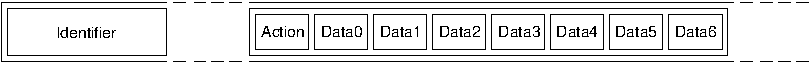
\includegraphics{../pics/protocol}}}
\end{center}
\caption{\label{fig:protokoll} Grunds�tzlicher Aufbau einer Nachricht zwischen
Bootloader und Programmiersoftware}
\end{figure}
\noindent Jeder Teilnehmer sendet alle seine Nachrichten unter
seinem Bezeichner (Identifier). Die Eindeutigkeit der Identifier 
aller Teilnehmer ist durch den Anwender sicher\-zu\-stellen. 
\newline
Die anderen beiden Elemente der Nachricht bedingen einander. Das mit 
{\it Action}\/ bezeichnete Feld enth�lt eine �bertragene Aktion, das 
nachfolgende Feld entsprechend Zusatzinformationen zu einer Aktion.
In Anlehnung an \cite{iar_bl}\/ sieht der Entwurf die folgenden Aktionen 
vor:
\begin{itemize}
        \item �ffnen
        \item Schlie�en
        \item Auswahl eines Speichers
        \item Auswahl einer Adresse
        \item L�schen eines Speichers
        \item Schreiben in einen Speicher
        \item Lesen aus einem Speicher
\end{itemize}
\noindent Die Programmiersoftware, im Folgendem auch kurz als Host bezeichnet,
ist der aktive Kommunikationspartner. Der Bootloader reagiert lediglich 
auf die empfangenen Nachrichten. Die Kommunikation 
l�uft nach dem Request-Response-Verfahren ab. Auf jeden Request vom Host 
erfolgt mindestens ein Response vom Bootloader. 
Die Inhalte der Request-Nachrichten und ihrer entsprechenden 
Response-Nachrichten sind im Einzelnen in Anhang \ref{anhang_protokoll}\/ 
aufgelistet. 
\newline
Entsprechend den genannten Aktionen, ist folgender
Programmablauf vorgesehen:
\begin{enumerate}
        \item Aktivieren der Bootloader\\
        Dieser initialen Aktion kommt besondere Bedeutung zu. In einem 
        Bussystem muss der Bootloader sicherstellen, dass s�mtliche 
        nachfolgende Befehle von genau einem Host stammen. Zu diesem Zweck 
        vermerkt ein Bootloader den aktivierenden Sender, und wird bis zum 
        Deaktivieren nur noch Befehle dieses Hosts akzeptieren. 
        \newline
        Im Einsatz mit mehreren Bootloadern kann der Umstand eintreten, 
        dass einige aktiviert sind, w�hrend andere auf eine Aktivierung warten.
        Um eine st�rungsfreie Kommunikation zwischen Host und aktivierten 
        Bootloadern zu gew�hrleisten, ignorieren nicht aktivierte Bootloader
        alle Aktionen bis auf diese. 
        \item Auswahl des Speichers\\
        Mikrocontroller k�nnen potentiell mehrere Speicher beinhalten, 
        beispielsweise Flash- oder EEPROM-Speicher. Adressen  
        k�nnen sich zwischen verschiedenen Speicherbereichen �berlappen.
        Daher wird vor nachfolgenden Aktionen 
        eine Auswahl notwendig. Voreingestellt ist der 
        Bereich des Flash-Speichers.
        \item Auswahl der Adresse\\
        Nachfolgende Aktionen k�nnen einzelne Adressbereiche eines 
        Speicherbereichs betreffen. In diesem Falle ist eine vorherige Angabe 
        notwendig. Voreingestellt ist Adresse 0.
        \item Ausf�hren des ISP\\
        Waren s�mtliche Aktionen bisher vorbereitend, wird nun das 
        eigentliche ISP durchgef�hrt. Sollen Daten geschrieben werden,
        erfolgt das �bertragen der Daten vom Host an die Bootloader. Werden  
        Daten gelesen, tauschen Host und die Bootloader die Rollen.
        Eine Erl�uterung dabei notwendiger steuernder Eingriffe wird sp�ter 
        gegeben. 
        \item Deaktivieren der Bootloader\\
        Als Abschluss werden die Bootloader f�r weitere Aktionen freigegeben.
\end{enumerate}
\noindent Das ISP kann zwischen Aktivieren und 
Deaktivieren wiederholte Vorbereitungen ben�tigen:
\begin{itemize}
        \item Komplettes L�schen\\
        Als Vorbereitung gen�gt die Auswahl des Speicherbereichs, der 
        gel�scht werden soll. 
        \item Schreiben\\
        Neben dem Speicherbereich ist auch die Adresse anzugeben, an der 
        geschrieben werden soll. Vorgesehen ist ein kontinuierlicher Modus,
        um den Overhead zu verringern. Damit gen�gt die Angabe einer 
        Startadresse. Alle empfangenen Daten werden kontinuierlich 
        an die nachfolgenden Adressen geschrieben.
        F�r nicht kontinuierlich aufeinander folgende Daten sind 
        zwischenzeitliche neue Adressangaben notwendig.
        \item Lesen\\
        Neben dem Speicherbereich ist die Adresse anzugeben, ab der Daten
        aus dem Speicher gelesen werden soll. Die Angabe der als letztes 
        zu lesenden Adresse erfolgt zusammen mit dem entsprechendem Befehl.
\end{itemize}
\noindent Wie eingangs erw�hnt, ist das Vorbild des entworfenen Protokolls in 
den L�sungen aus Abschnitt \ref{l:atmel_bl}\/ zu finden. Wesentlicher 
Unterschied ist die 
Verwendung des 
Bezeichners einer CAN-Nachricht zur Individualisierung. Damit einher geht auch
die Verringerung der Nutzlast einer CAN-Nachricht. Ein Datenbyte muss nun f�r 
die Kennzeichnung der Aktion verwendet werden. Der verwendete 
Request-Response-Ansatz erleichtert die Implementierung, muss jedoch als  
langsam bewertet werden.

%Interrupts. CAN-Treiber. 
%asynchron. microkernel-konzept, da shm eh ben�tigt.
% bl-support bietet alle m�glichkeiten
% modular
% schnittstelle zum can, isp: weil unterschiedlich
% protokoll selber trennen. kein monolith, sondern aufgabenspezifisch
\subsection{Bootloader}
\label{l:bootloader}
Ausgangspunkt f�r den Entwurf des Bootloaders 
war die Abstraktion von der zugrunde liegenden Hardware. So konnten h�here 
Programmfunktionen unabh�ngig entworfen werden, 
zugleich wird die Portierung auf andere Hardware vereinfacht.
Wie aus Abschnitt \ref{l:protokoll}\/ ersichtlich, l�sst sich das verwendete 
Protokoll auch mit anderen Schnittstellen verwenden. Der Entwurf musste auch
dies ber�cksichtigen. 
Zusammengefasst ergab sich die Forderung nach m�glichst unabh�ngigen 
Komponenten. 
\newline
Aus der Funktionsweise des ISP wird ersichtlich, dass mit einem 
lokalen Puffer gearbeitet werden muss. In diesem sind m�glicherweise zu 
lesende Daten zu speichern. Aus Gr�nden der Performance ist es sinnvoll, 
auch schreibende Daten zu puffern. Vor diesem Hintergrund bietet sich die 
M�glichkeit an, alle Komponenten lediglich �ber Puffer miteinander 
kommunizieren zu lassen. Die Verbindung zwischen den Komponenten wird �ber 
Nachrichten hergestellt, welche �ber eine zentrale Instanz verteilt werden.
Abbildung \ref{fig:komp_diagram_shumway}\/ zeigt das Komponentendiagramm des 
Entwurfs.
\begin{figure}[htbp]
\begin{center}
        \scalebox{1.0}{\rotatebox{270}{\includegraphics{../pics/komp_model_shumway}}}
\end{center}
\caption{\label{fig:komp_diagram_shumway} Komponentendiagramm des Bootloader}
\end{figure}
\noindent Die funktionalen Komponenten des Entwurfs, die Server, kommunizieren
untereinander �ber die mit Kernel bezeichnete Instanz. Dazu signalisieren sie
dem Kernel eine ausgehende Nachricht, dieser dann entsprechend 
weiter reicht. Ein Server kennzeichnet eine Nachricht durch eine Richtung.
Entweder die Nachricht soll in der Serverhierarchie nach oben wandern oder 
nach unten. Bei Unklarheit �ber die Hierarchie wird die Richtung entsprechend 
als unbekannt definiert.
\newline
Ist kein Empf�nger f�r ein Signal existent, wird der Sender benachrichtigt.
Dadurch wird es m�glich, unabh�ngig von der jeweiligen Konfiguration 
zu bleiben. Ist beispielsweise kein Debugging gew�nscht, wird der zust�ndige 
Server aus dem System genommen. Derzeit wird dies lediglich zur 
Kompilierzeit get�tigt. Ein Entfernen auch zur Laufzeit sollte im Bedarfsfall
keinen gro�en Aufwand erfordern. Weiterhin wird die Nutzung 
von Interrupts m�glich. Anstatt an verschiedenen Punkten auf 
externe Ereignisse zu pollen, braucht mit dem Kernel lediglich 
eine zentrale Instanz auf nun interne Ereignisse zu pollen. 
Interne Ereignisse sind die Nachrichten, die von den einzelnen Servern, 
m�glicherweise in Reaktion auf Interrupts, signalisiert werden. 
\newline
Die Nachteile dieses Entwurfs sind eine verringerte Geschwindigkeit und 
ein erh�hter Speicherbedarf. Letzteres ist aufgrund der Anforderungen unbedingt
w�hrend der Implementation zu beachten.



%auf avrdude-seite. lex/yacc config. autoconfigure.  vorgegebenes 
%programmer-struct
\subsection{Programmiersoftware}
Aufgrund vorheriger Erfahrungen und der angebotenen M�glichkeiten wurde sich
f�r eine Erweiterung der in Abschnitt \ref{l:avrdude}\/ genannten 
Programmiersoftware {\it Avrdude}\/ entschieden. Die Schnittstelle und die 
Anwendung
bleiben daher f�r bisherige Benutzer gleich. Auf Entwurfseite konnte auf das 
Handling mit Dateien und das Benutzerinterface verzichtet werden.
\newline
Ohne Anspruch auf Vollst�ndigkeit, gibt Abbildung 
\ref{fig:komp_diagram_avrdude}\/ einen �berblick �ber die Komponenten von 
{\it Avrdude}\/.
\begin{figure}[htbp]
\begin{center}
        \scalebox{1.0}{\rotatebox{0}{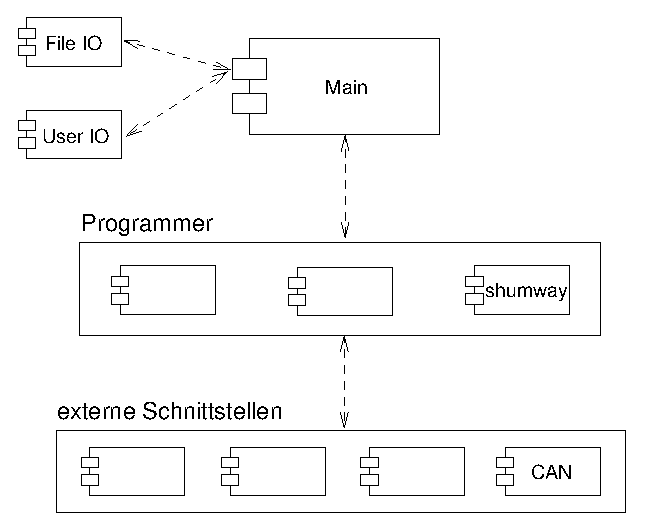
\includegraphics{../pics/komp_model_avrdude}}}
\end{center}
\caption{\label{fig:komp_diagram_avrdude} Komponentendiagramm von Avrdude}
\end{figure}
\noindent Ersichtlich wird, dass eine Erweiterung sich auf zwei neue 
Komponenten beschr�nken kann.
Zun�chst ist es notwendig, eine zus�tzliche Schnittstelle f�r den 
CAN-Bus zu entwickeln. Die Funktionalit�t kann sich dabei an den bereits 
existierenden Schnittstellen orientieren. Weiterhin muss ein neuer
Programmer entwickelt werden. Dieser stellt, auf h�herer Ebene, den 
Adapter zwischen {\it Avrdude}\/ und einem verwendetem Befehlprotokoll dar. 
S�mtliche
spezifische Funktionalit�t bleibt in dieser Komponente gekapselt. Daher kann 
auch die Unterst�tzung f�r mehrere Kommunikationspartner in dieser Komponente
realisiert werden.


%klassendiagramm.
%\section{Implementierung}
%\subsection{Botloader}
%benutzung avr-gcc. c++. hilfsmittel. 
%problem mit avr-gcc. 
%\subsection{Pogrammiersoftware}
%c auf avrdude-seite, da vorgegeben. verwendung peak can-library. 
%problem dabei.
%klassendiagramm.
\section{Implementierung}
Die Umsetzung des Entwurfs aus Abschnitt \ref{l:entwurf}\/ umfasste den 
Bootloader sowie das Gegenst�ck auf Seite des PC. 
Wesentlicher Teil der jeweiligen Implementation war die Unterst�tzung des 
in Abschnitt \ref{l:protokoll}\/ erl�uterten Protokolls.

%benutzung avr-gcc. c++. hilfsmittel. 
%problem mit avr-gcc. 
\subsection{Bootloader}
Zur Implementierung des Bootloaders wurde sich f�r die Verwendung 
der in Abschnitt \ref{l:avr_se}\/ genannten M�glichkeiten entschieden. Das 
erlaubte zwischenzeitliche Funktionstests ohne zus�tzlichen 
Aufwand, wurde doch unter dem gleichen Betriebssystem entwickelt wie in der 
sp�teren Anwendung.
\newline
Die Wahl der Programmiersprache fiel auf C++. Mit Verwendung 
dieser Sprache wurde
es m�glich, f�r h�here Programmfunktionalit�t einen objektorientierten
Ansatz zu verwenden. Entsprechend konnte die Struktur �bersichtlich 
gehalten werden. Zu beachten waren Nachteile bez�glich des Umfangs des 
Programmcode, resultierend aus automatisch generiertem Code, beispielsweise f�r
Konstruktoren oder Destruktoren. 
Mit C++ wurde es gleichzeitig m�glich, f�r die untere
Programmfunktionalit�t reine C-Implementationen zu verwenden. 
Dies betraf die Schnittstellen zur Hardware.
Hier wurde der imperative Ansatz von C bez�glich Einfachheit und 
Ressourcenbedarf als vorteilhaft eingesch�tzt.
\newline
In Fortf�hrung des Entwurfs aus Abschnitt \ref{l:bootloader} ergab sich 
eine aus verschiedenen Klassen bestehende Architektur.
Aus Gr�nden der �bersichtlichkeit werden die entsprechenden Klassendiagramme
geteilt. Abbildung \ref{fig:klass_dia_server}\/ stellt die Architektur der
Server dar. 
\begin{figure}[htbp]
\begin{center}
        \scalebox{1.0}{\rotatebox{270}{\includegraphics{../pics/klass_dia_server-crop}}}
\end{center}
\caption{\label{fig:klass_dia_server} Klassendiagramm der Server}
\end{figure}
\noindent Wie im Entwurf erl�utert, beinhalten diese die eigentliche 
Funktionalit�t. Zu sehen ist, dass die Server untereinander 
minimal gekoppelt sind. Alle verwenden einen gemeinsamen Speicher, von dem sie
bei Bedarf Teile reservieren, bearbeiten und wieder freigeben. Inhalt der 
Teile sind im Normalfall Nachrichten an andere Server, aber auch zu schreibende
oder gelesene Daten aus bzw. von Bereichen des Programmspeichers. Das 
Befehlprotokoll wird nur innerhalb der {\it receive}\/-Routine realisiert. 
Aufgrund der Anzahl der verschiedenen Befehle vollzieht diese Routine im 
Wesentlichen eine Fallunterscheidung. 
\newline
Das angewandte Mediator-Pattern setzt sich in den in Abbildung 
\ref{fig:klass_dia_kernel}\/ dargestellten Elementen fort.
\begin{figure}[htbp]
\begin{center}
        \scalebox{1.0}{\rotatebox{270}{\includegraphics{../pics/klass_dia_kernel-crop}}}
\end{center}
\caption{\label{fig:klass_dia_kernel} Klassendiagramm des Kernel}
\end{figure}
\noindent 
Die Server kommunizieren untereinander durch das Signalisieren von Nachrichten
an den Kernel. Wie bereits angedeutet, k�nnen einzelne Server in Reaktion auf 
Interrupts selbstst�ndig aktiv werden. Zu diesem Zweck bieten derartige Server
statische Einstiegspunkte f�r Interrupt Service Routinen. Um in einem 
solchen Fall mit anderen Servern kommunizieren zu k�nnen, m�ssen die
nebenl�ufig generierten Nachrichten zwischengespeichert werden. 
Diesem Zweck dient die Queue des Kernels.
Deren Abarbeitung nimmt der Kernel innerhalb einer Endlosschleife vor. Liegt 
eine Nachricht vor, wird der passenden Server gesucht und dessen 
{\it receive}\/-Routine aufgerufen. Nach Beendigung der Routine wird die 
n�chste Nachricht abgearbeitet usw. 
Dementsprechend erfolgt die Abarbeitung der Nachrichten streng in einem
Thread. Nachrichten selbst k�nnen wiederum beim Abarbeiten einer Nachricht
in die Queue gestellt werden. Dies kann aber auch, wie beschrieben, in 
Reaktion auf einen Interrupt geschehen.
\newline
Die Namen der einzelnen Server geben deren Aufgaben wieder. Der Server 
{\it S\_Can\_Phy}\/ bildet die Schnittstelle zum CAN-Bus. Nachrichten auf dem 
Bus werden
interruptgesteuert an den Kernel signalisiert. Umgekehrt realisiert das
Abarbeiten einer Nachricht das Versenden von Daten und die Steuerung der
CAN-Schnittstelle. Der Server {\it S\_Id}\/ agiert als Filter f�r Nachrichten, 
die vom CAN-Bus stammen. Das ISP wird von Server {\it S\_Isp}\/ durchgef�hrt. 
Beinahe das gesamte Befehlprotokoll der Entwicklung ist in diesem Server
realisiert. Das Schreiben bzw. L�schen eines Programmspeichers wird 
ebenfalls interruptgesteuert vorgenommen. Die derzeitige Implementierung 
verlangt jedoch ein Warten der weiteren Abarbeitung, bis ein ISP-Vorgang
abgeschlossen ist. Der Server {\it S\_Timer}\/ dient dem Start einer 
Applikation nach Ablauf einer vorgegebenen Zeitspanne.
\newline
Von der Darstellung der in C implementierten Funktionalit�t wird
abgesehen. Diese sind eng mit der Hardware verkn�pft. Eine allgemeine 
Architektur l�sst sich hier nicht angeben. Es war jedoch nicht Ziel der Arbeit,
f�r die hardwarenahe Funktionalit�t eine allgemeine Architektur zu realisieren.


%c auf avrdude-seite, da vorgegeben. verwendung peak can-library. problem 
% dabei.
\subsection{Programmiersoftware}
Aufgrund der Erweiterung von {\it Avrdude}\/ war die Art und Weise der 
Implementierung bereits vorgegeben. So musste die Programmiersprache C 
verwendet werden. Die API von {\it Avrdude}\/ legte die zu implementierenden 
Routinen bereits fest.
\newline
Zentrales Element der API ist eine mit {\it PROGRAMMER}\/ 
bezeichnete Struktur. Diese wird durch Scannen und Parsen eines Config-Files
f�r die sp�tere Verwendung vorbereitet. Zum Einsatz kommen daf�r die 
unter {\mbox Linux}\/ klassischen Programme {\it lex}\/ und {\it bison}\/.
Im Anschluss beinhaltet die {\it PROGRAMMER}\/-Struktur - unter anderem - 
Zeiger auf spezifische Routinen. {\it Avrdude}\/ geht im eigentlichem 
Programmlauf
nun entsprechend seines Algorithmus' vor. �ber die {\it PROGRAMMER}\/-Struktur
werden spezifische Routinen aufgerufen, wann immer der allgemein g�ltige Pfad
verlassen wird.
\newline
Neben den obligatorischen Routinen wurden in der Erweiterung 
zwei Routinen zum Schreiben und Lesen implementiert. 
S�mtliche neuen Routinen wurden in der direkt f�r {\it Avrdude}\/ sichtbaren 
Komponente {\it Shumway}\/ zusammengefasst. Der Name der Komponente ist das
Resultat eines Wortspiels. Daran beteiligt sind der Zweck der Erweiterung, 
das Flashen, und die Namen der Hauptfiguren zweier Fernsehserien, 
Flash Gordon und Gordon Alf Shumway.
\newline
S�mtliche Aufrufe gehen �ber die zweite
entwickelte Komponente, der Schnittstelle zum CAN-Bus.
Abbildung \ref{fig:dia_avrdude}\/ gibt einen Einblick in beide Komponenten.
\begin{figure}[htbp]
\begin{center}
        \scalebox{1.0}{\rotatebox{270}{\includegraphics{../pics/dia_avrdude}}}
\end{center}
\caption{\label{fig:dia_avrdude} Struktur der Erweiterung von Avrdude}
\end{figure}
\newline
Die Implementierung der Schnittstelle zum CAN-Bus versucht, die Trennung vom
verwendetem Treiber zumindest vorzubereiten. 
Gem�� den Anforderungen wurde die {\it libpcan}\/ f�r die 
Implementation verwendet. Abweichend vom unter Unix �blichen Filedescriptor,
benutzt diese Bibliothek ein eigenes Konstrukt zur Beschreibung einer
Schnittstelle. Im Zusammenspiel mit {\it Avrdude}\/ ergab sich damit ein
Problem.
Wie schon erw�hnt, ruft {\it Avrdude}\/ spezifische Routinen 
entsprechend seinem Ablauf ab. Eine einmal ge�ffnete externe Schnittstelle 
muss daher zwischengespeichert werden. Dies geschieht in der
{\it PROGRAMMER}\/-Struktur, welche den �blichen Filedescriptor 
beinhaltet. Das Konstrukt der {\it libpcan}\/, das sog. Handle, beinhaltet 
seinerseits einen Filedescriptor, so dass ein Zwischenspeichern m�glich ist.
Jedoch erwarten s�mtliche Routinen der {\it libpcan}\/ ein Handle als 
Argument, ein Filedescriptor wird nicht unterst�tzt.
Ein zus�tzliches Mapping zwischen beiden Konstrukten 
ist daher notwendig. Wie aus Abbildung \ref{fig:dia_avrdude}\/ ersichtlich, 
wurde dies in der f�r die {\it libpcan}\/ spezifischen Implementation 
realisiert. Damit konnte das Interface von {\it Avrdude}\/ zur 
CAN-Schnittstelle unabh�ngig von der Implementation gehalten werden.









 



%\section{Anwendung}
%auspielen bootloader per fremdem programmer. verwendung avrdude wie bekannt.
%m�glichkeiten verbosity.
%was geht nicht.
%aufspielen bootloader per fremdem programmer. verwendung avrdude wie bekannt.
%m�glichkeiten verbosity.
%schnelligkeit
%was geht nicht.
\section{Anwendung}
\label{l:anwendung}

Vor einer Anwendung der entwickelten L�sung sind mehrere Schritte notwendig. 
Zun�chst m�ssen die Quellen in ausf�hrbaren Programmcode �bersetzt werden. 
Anschlie�end m�ssen die Programme installiert werden.
Waren beide Schritte erfolgreich, kann schluss\-endlich die Anwendung erfolgen.

\subsection{Einrichten und �bersetzen}
\label{l:uebers}
Zum �bersetzen des Bootloaders sollte das beiliegende Makefile verwendet 
werden. Der Pfad zum Compiler ist ggf. in der Variable {\it DIRAVR}\/ zu 
setzen.
Zwei Einrichtungsaufgaben sind durchzuf�hren:
\begin{itemize}
        \item Einstellen der Baudrate\\
        Fest einzustellen ist die Baudrate, mit welcher der Bootloader auf 
        dem CAN-Bus kommuniziert. Dazu sind in  der
        Datei \glqq config.h\grqq\/ im Verzeichnis \glqq config\grqq\/ die 
        Einstellungen f�r die entsprechenden {\it CANBT}\/-Register zu 
        treffen. Voreingestellt ist eine Baudrate von 250 kbit/s.
        \item Einstellen des Bezeichners\\
        Wie in Abschnitt \ref{l:protokoll}\/ erl�utert, muss jeder 
        Teilnehmer einen eindeutigen Bezeichner besitzen. Dazu ist die Routine
        {\it get\_own\_id()}\/ aus der Datei \\
        \glqq board\_drv\_ktb\_can128.h\grqq\/, zu finden unter
        \glqq lib/board\grqq\/, entsprechend anzupassen. Im Bedarfsfall 
        k�nnen eigene Befehle zur Festlegung des Bezeichners eingebracht 
        werden.
\end{itemize}
F�r das �bersetzen von {\it Avrdude}\/ wird auf die der Software beiliegenden 
Dokumentation verwiesen. Die get�tigte Erweiterung hat keinen Einfluss 
auf das dort erl�uterte Vorgehen.
Explizit zu nennende Einrichtungsaufgaben sind nicht bekannt.

\subsection{Installieren}
\label{l:inst}
Das Installieren des Bootloaders beschr�nkt sich auf das �bertragen des
Programmcode auf den Mikrocontroller. Dazu kann eine beliebige 
Programmiersoftware, beispielsweise auch {\it Avrdude}\/, verwendet
werden. Die Prozedur unterscheidet sich im Einzelnen je nach 
Programmiersoftware und Programmieradapter. Bei Verwendung von {\it Avrdude}\/
in
Verbindung mit einem STK200-kompatiblen Adapter lautet der Aufruf 
beispielsweise wie folgt:
\begin{verbatim}
avrdude -p at90can128 -P /dev/parport0 -c stk200 -U flash:w:shumway.hex
\end{verbatim}
Dieser Befehl spricht einen AT90CAN128 �ber einen am ersten 
Parallelport befindlichen Adapter an.
\newline
Abschlie�end ist durch Setzen der Fuse-Bits sicherzustellen, dass nach einem
Reset der Bootloader korrekt gestartet wird. F�r den AT90CAN128 bedeutet dies 
ein L�schen der drei niederwertigsten Bits des Fuse-High-Bytes. Soweit bekannt,
kann dies ebenfalls mit g�ngiger Programmiersoftware erreicht werden. Analog
zu obigem Beispiel, lautet der Aufruf von {\it Avrdude}\/ dazu:
\begin{verbatim}
avrdude -p at90can128 -P /dev/parport0 -c stk200 -U hfuse:w:0xD8:m
\end{verbatim}
Die verwendete Bitmaske 0xD8 entspricht den Standardeinstellungen.
\newline
F�r die Installation von {\it Avrdude}\/ wird abermals auf die der Software 
beiliegenden Dokumentation verwiesen. 

\subsection{Anwendung}
\label{l:benutz}
F�r den Anwender beschr�nkt sich die Anwendung auf die Bedienung von 
{\it Avrdude}\/.
Aus diesem Grunde ist auch hier die Dokumentation zu diesem Programm 
hilfreich. 
\newline
Die Konfiguration von {\it Avrdude}\/ ist in der Datei \glqq avrdude.conf
\grqq\/
vorzunehmen. Mehrere Einstellungen betreffen die Erweiterung.
\begin{itemize}
        \item {\it default\_can}\/\\
        Dies ist die Festlegung der voreingestellten Schnittstelle zum 
        CAN-Bus. Fehlt beim Aufruf von {\it Avrdude}\/ die Angabe der 
        Schnittstelle,
        wird die hier aufgef�hrte Schnittstelle verwendet. Voreingestellt ist 
        die Schnittstelle {\it /dev/pcan24}\/, die f�r die in den
         Anforderungen genannten PCAN-Dongles zutreffend ist.
        \item {\it can\_id\_host}\/\\
        Wie die Bootloader, muss auch {\it Avrdude}\/ einen 
        eindeutigen Bezeichner f�r Nachrichten auf dem CAN-Bus verwenden. 
        Mit dieser Einstellung wird der Bezeichner festgelegt.
        Voreingestellt ist der Wert 0.
        \item {\it can\_use\_ext\_id}\/\\
        Diese Einstellung erm�glicht die Benutzung von erweiterten Bezeichnern
        auf dem CAN-Bus. Da der Bootloader dies zwingend fordert, ist
        eine Anwendung bisher nicht m�glich und die Einstellung m�glichen
        Weiterentwicklung vorbehalten. Der Wert ist unbedingt auf der 
        Voreinstellung 'yes' zu belassen.
        \item {\it can\_expected\_nodes\_num}\/\\
        F�r das Programmieren wurde auf eine individuelle Adressierung
        verzichtet. Daher bleibt die Anzahl der angesprochenen 
        Mikrocontroller zun�chst {\it Avrdude}\/ �berlassen. Dies kann der 
        eigentlichen Absicht des Anwenders widersprechen. Unter Umst�nden
        befinden sich irrt�mlich Mikrocontroller im Bootloader-Modus,
        f�r welche der anlaufende Programmiervorgang nicht gedacht ist.
        F�r diesen Fall kann mit dieser Einstellung 
        die Anzahl der erwarteten Mikrocontroller 
        vorgegeben werden. Stellt {\it Avrdude}\/ den Kontakt mit mehr oder 
        mit 
        weniger Mikrocontrollern her, wird der Programmiervorgang nicht 
        gestartet. Die Voreinstellung von 0 weist {\it Avrdude}\/ an, keine 
        Vorgabe zu verwenden. Somit werden alle Mikrocontroller programmiert,
        zu denen der Kontakt hergestellt werden konnte.
\end{itemize}
\noindent
Der Name des von {\it Avrdude}\/ zu verwendenden Programmieradapters lautet 
'pcan'.
Insgesamt wird das Programmieren durch folgenden Aufruf von {\it Avrdude}\/ 
gestartet:
\begin{verbatim}
avrdude -p at90can128 -c pcan -U flash:w:<datei>
\end{verbatim}
Anstelle des Speicherbereichs Flash kann auch der Speicherbereich EEPROM
gew�hlt werden. F�r diesen Fall lautet der Aufruf von {\it Avrdude}\/:
\begin{verbatim}
avrdude -p at90can128 -c pcan -U eeprom:w:<datei>
\end{verbatim}
So genannte Verbose-Optionen k�nnen {\it Avrdude}\/ dazu auffordern, mehr 
Informationen �ber den
Programmlauf zu liefern. Nach der Anzahl der verwendeten Optionen lassen
sich vier Stufen der Ausgabe unterschieden. 
\begin{list}{}{}
        \item{0 -} Keine zus�tzliche Ausgabe von Informationen.
        \item{1 -} Aufgetretene Fehler werden weiter erl�utert.
        \item{2 -} Informationen �ber den Programmlauf werden ausgegeben.
        \item{3 -} Ausgabe von Informationen der verwendeten Schnittstelle.
\end{list}
Die Stufen bauen aufeinander auf, eine Stufe beinhaltet somit alle 
vorhergehenden. In der normalen Anwendung sollte sich jedoch die Verwendung der
Verbose-Optionen er�brigen. Eine beispielhafte Ausgabe von {\it Avrdude}\/ 
ist in Anhang \ref{anhang_avrdude}\/ aufgef�hrt.
\newline
\newline
Wie in \ref{l:funkt}\/ gefordert, sollte f�r programmierte Mikrocontroller die
M�glichkeit bestehen, ohne Reset ein erneutes Programmieren zu erm�glichen.
Zu diesem Zweck muss eine laufende Mikrocontroller-Anwendung an 
eine vorbereitete Adresse springen. F�r eine bequeme Implementierung 
einer derartigen Funktionalit�t wurde die Routine 'loader\_run()' vorbereitet.
Diese befindet sich in der Header-Datei 'loader.h', zu finden
im Verzeichnis 'frame' im Quellcode des Bootloader. Eine Anwendung f�r den 
Mikrocontroller braucht lediglich diese Header-Datei einzubinden. 
Nach erfolgreichem Kompilieren und Programmieren kann zur 
Laufzeit der Anwendung die genannte Routine aufgerufen werden, um ein 
erneutes Programmieren zu erm�glichen.

\subsection{Evaluation}
\label{l:eval}
Im Folgendem soll ein Einblick in die Geschwindigkeit des 
Programmiervorgangs gegeben werden.
F�r den Erhalt der Angaben wurde jeweils ein 
Programmiervorgang mit zwei angeschlossenen Mikrocontrollern durchgef�hrt.
Die auf dem CAN-Bus verwendete Baudrate betrug 250kbit/s. S�mtliche Werte sind lediglich Richtwerte und sollen die zu erwartenden Zeiten verdeutlichen.
\newline
Tabelle \ref{tab:eval}\/ gibt die Zeiten f�r das Schreiben in den 
Flash-Speicher der Mikrocontroller an.
\begin{table}[htbp]
\centering
\begin{tabularx}{0.9\linewidth}{|c|Y|Y|Y|}
\hline
Anzahl Daten & Zeit f�r L�schen & Zeit f�r Schreiben & Zeit f�r Verify \\ \hline
2090 Bytes & 2,3s & 1,50s & 1,63s \\
67626 Bytes & 2,3s & 44,38s & 51,73s\\
120874 Bytes & 2,3s & 79,65s & 93,60s\\
\hline
\end{tabularx}
\caption{\label{tab:eval}Zu erwartende Zeiten f�r den Programmiervorgang des Flash-Speichers}
\end{table}
\noindent 
Die Zeit zum L�schen bleibt konstant, da dies eine selbstst�ndige Aktion der
Mikrocontroller ist. Die daf�r ben�tigte Zeit ist durch die Hardware 
vorgegeben.
\newline
In Tabelle \ref{tab:eval_eeprom}\/ sind die Zeiten aufgelistet, wie sie f�r 
das Schreiben in den EEPROM-Speicher zu erwarten sind.
\begin{table}[htbp]
\centering
\begin{tabularx}{0.9\linewidth}{|c|Y|Y|Y|}
\hline
Anzahl Daten & Zeit f�r L�schen & Zeit f�r Schreiben & Zeit f�r Verify \\ \hline
64 Bytes & 34,8s & 0,61s & 0,11s \\
2128 Bytes & 34,8s & 19,33s & 1,71s\\
3792 Bytes & 34,8s & 34,37s & 3,04s\\
\hline
\end{tabularx}
\caption{\label{tab:eval_eeprom}Zu erwartende Zeiten f�r den Programmiervorgang des EEPROM-Speichers}
\end{table}
\noindent
Auch hier ist die Zeit zum L�schen von der Hardware bedingt. Wie zu sehen ist, 
sind Schreibzugriffe auf das EEPROM sehr langsam. Auch ist die Anzahl 
garantierter Schreib- bzw. L�schzyklen vergleichsweise gering. Die 
Implementierung ber�cksichtigt diese Umst�nde, indem nur geschrieben wird, 
wenn dies erforderlich ist. Sind zu schreibende Werte bereits im EEPROM 
vorhanden, wird auf diesem Wege Zeit gespart und die Lebensdauer erh�ht. 
Die angegebenen Werte sind als Maximalwerte zu betrachten, da sie 
auf einem vorher gel�schten EEPROM beruhen.
\newline
{\it Avrdude}\/ versucht, vor dem Schreiben in den Flash-Speicher alle 
Speicherbereiche
eines Mikrocontrollers zu l�schen. Im Rahmen dieses sog. Chip-Erase betrifft
das auch den EEPROM-Speicher. Dazu sind jedoch im schlechtesten Fall
mehr als 34 Sekunden notwendig.
Einem Anwender, der lediglich das Flash beschreiben will, ist diese 
Wartezeit nicht zuzumuten. Daher wurde der Bereich EEPROM vom Chip-Erase 
ausgenommen. Da bedeutet auch, dass der EEPROM-Speicher nicht gel�scht werden 
kann. Selbstverst�ndlich k�nnen aber neue Daten abgelegt werden.
\newline
Im Vergleich zur herk�mmlichen Programmierung sind die Zeiten f�r den 
EEPROM-Speicher ann�hernd gleich. Lediglich im Verify werden wenige Sekunden
zus�tzlich ben�tigt. F�r den Bereich des Flash-Speichers halbiert
sich die Geschwindigkeit nahezu. Die Gr�nde daf�r konnten bis zum Abschluss 
der Arbeit nicht gekl�rt werden. 
Das verwendete Request-Response-Verfahren ist sicherlich kein 
schnelles Verfahren. Auf jeweils sieben Bytes Daten muss eine Best�tigung 
versandt und abgewartet werden. Der CAN-Bus sollte aufgrund der 
verwendeten Baudrate keinen Engpass darstellen. Die H�ufigkeit der 
auf den Mikrocontrollern laufenden ISP-Prozeduren hat ebenfalls nur geringen 
Einfluss. Versuche mit unterschiedlichen Puffergr��en sind zu diesem 
Zwecke erfolgt. Auf Seite von {\it Avrdude}\/ sind keine bedeutenden 
Verz�gerungen bekannt. Ein Wechsel der verwendeten Bibliothek f�r die 
CAN-Schnittstelle ist aufgrund der Anforderungen nicht m�glich. Als 
bedeutende Ursache 
vermutet wird eine lange Verarbeitungszeit auf dem Mikrocontroller, bedingt 
durch das vielfache Message-Handling. Ein direktes Mapping zwischen den 
Servern, welches m�glicherweise einen schnelleren Ablauf bewirken w�rde,
konnte mangels Speicherplatz nicht eingesetzt werden. Denkbar ist weiterhin, 
dass das h�ufige Warten auf den Abschluss eines ISP-Vorgangs Zeit kostet. 
Ein erster Test konnte diese Vermutung jedoch nicht best�tigen.

% 250000 bit/s = 1602 can-nachrichten bei vollen 156 bit
% angenommen, nur die h�lfte daten, der rest ack's
% entspricht 5610 byte/s daten hin. ben�tigt daher f�r 120874 21,5 sekunden
% aber 79s gemessen
 
 






%\section{Zusammenfassung und Ausblick}
%was wurde gemacht. was wurde nicht gemacht und warum nicht. was k�nnte/sollte 
%davon noch gemacht werden
%was wurde gemacht. was wurde nicht gemacht und warum nicht. was k�nnte/sollte 
%davon noch gemacht werden
% funktioniert. verwendung avrdude passt sich in bisherige arbeitsweise ein
% nur flash, weil kein platz mehr
% langsam
% zuk�nftig? eeprom, daf�r aber platz schaffen notwendig. fuses, ebenso
\section{Zusammenfassung und Ausblick}
\label{l:zus_ausbl}
Mit der entwickelten L�sung ist es m�glich, gleichzeitig mehrere 
Mikrocontroller der AT90CAN-Baureihe �ber deren CAN-Schnittstelle zu 
programmieren. Dem Benutzer wird mit der Erweiterung des Programms 
{\it Avrdude}\/ ein entsprechendes Werkzeug zur Anwendung gegeben. 
Die gesamte Entwicklung erfolgte unter Verwendung von offen gelegter Software
unter dem Betriebssystem Linux. Da Avrdude den Quasi-Standard f�r 
Programmiersoftware unter Linux darstellt, wird der  
Aufwand zur Anwendung als minimal angenommen.
\newline
Nicht realisiert wurden M�glichkeiten zum Programmieren
der Fuse-Bytes. Ebenso fehlt ein eigener Update-Mechanismus. 
Die Entwicklung 
der genannten Punkte scheiterte am verf�gbaren Speicherplatz. Allerdings kann 
aufgrund der Architektur der L�sung angenommen werden, dass entsprechende 
Modifikationen einfach durchf�hrbar sind. Ob eine Variante 
jemals alle Bereiche programmieren kann, oder aber verschiedene spezialisierte 
Varianten existieren, wird nicht zuletzt durch den Bedarf entschieden.
Gleiches trifft auch f�r Verbesserungen hinsichtlich der 
Performance zu.




%\cleardoublepage
\appendix
\phantomsection
\addcontentsline{toc}{part}{\appendixname}

\section{Befehlprotokoll}
\label{anhang_protokoll}
%Anhang mit Progs
\pagestyle{appendix_deep}


\subsection{�ffnen}
        \begin{table}[htbp]
        \centering
        \begin{tabularx}{0.9\linewidth}{|c|c|Y|}
        \hline
        {\bf Aktion} & {\bf Daten} & {\bf Beschreibung} \\ \hline
        SELECT\_OPEN & - & �ffnet Empf�nger f�r weitere Nachrichten von 
        diesem Sender\\
        \hline
        \end{tabularx}
        \caption{\label{tab:so_req}Anfrage des Hosts nach �ffnen}
        \end{table}
        \begin{table}[htbp]
        \centering
        \begin{tabularx}{0.9\linewidth}{|c|c|Y|}
        \hline
        {\bf Aktion} & {\bf Daten} & {\bf Beschreibung} \\ \hline
        SELECT\_OPEN & OK & Empf�nger f�r weitere Nachrichten von diesem
        Sender bereit\\
        \hline
        SELECT\_OPEN & ERROR & Empf�nger konnte ungest�rten weiteren 
        Empfang nicht sicherstellen\\
        \hline
        \end{tabularx}
        \caption{\label{tab:so_resp}Antwort des Bootloaders auf �ffnen}
        \end{table}

\subsection{Schlie�en}
        \begin{table}[htbp]
        \centering
        \begin{tabularx}{0.9\linewidth}{|c|c|Y|}
        \hline
        {\bf Aktion} & {\bf Daten} & {\bf Beschreibung} \\ \hline
        SELECT\_CLOSE & - & Beenden des Empfangs weiterer Nachrichten 
        dieses Senders\\
        \hline
        \end{tabularx}
        \caption{\label{tab:sc_req}Anfrage des Hosts nach Schlie�en}
        \end{table}
        \begin{table}[htbp]
        \centering
        \begin{tabularx}{0.9\linewidth}{|c|c|Y|}
        \hline
        {\bf Aktion} & {\bf Daten} & {\bf Beschreibung} \\ \hline
        SELECT\_CLOSE & OK & Empf�nger geschlossen\\
        \hline
        \end{tabularx}
        \caption{\label{tab:sc_resp}Antwort des Bootloaders auf Schlie�en}
        \end{table}


\subsection{Speicherwahl}
        \begin{table}[htbp]
        \centering
        \begin{tabularx}{0.9\linewidth}{|c|c|Y|}
        \hline
        {\bf Aktion} & {\bf Daten} & {\bf Beschreibung} \\ \hline
        MEM\_SELECT & MEM & Auswahl einer Speichers f�r weitere Aktionen\\
        \hline
        \end{tabularx}
        \caption{\label{tab:ms_req}Anfrage des Hosts nach Wahl eines Speichers}
        \end{table}
        \begin{table}[htbp]
        \centering
        \begin{tabularx}{0.9\linewidth}{|c|c|Y|}
        \hline
        {\bf Aktion} & {\bf Daten} & {\bf Beschreibung} \\ \hline
        MEM\_SELECT & OK & Speicherwahl erfolgreich\\
        \hline
        MEM\_SELECT & ERROR & Speicherwahl ung�ltig\\
        \hline
        \end{tabularx}
        \caption{\label{tab:ms_resp}Antwort des Bootloaders auf Wahl des Speichers}
        \end{table}

\pagebreak

\subsection{Adresswahl}
        \begin{table}[h]
        \centering
        \begin{tabularx}{0.9\linewidth}{|c|c|Y|}
        \hline
        {\bf Aktion} & {\bf Daten} & {\bf Beschreibung} \\ \hline
        ADDR & Adresse & Auswahl einer Adresse f�r weitere Aktionen\\
        \hline
        \end{tabularx}
        \caption{\label{tab:as_req}Anfrage des Hosts nach Wahl der Adresse}
        \end{table}
        \begin{table}[h]
        \centering
        \begin{tabularx}{0.9\linewidth}{|c|c|Y|}
        \hline
        {\bf Aktion} & {\bf Daten} & {\bf Beschreibung} \\ \hline
        ADDR & OK & Adresswahl erfolgreich\\
        \hline
        ADDR & ERROR & Adresswahl ung�ltig\\
        \hline
        \end{tabularx}
        \caption{\label{tab:as_resp}Antwort des Bootloaders auf Wahl der Adresse}
        \end{table}

\subsection{Speicher komplett l�schen}
        \begin{table}[h]
        \centering
        \begin{tabularx}{0.9\linewidth}{|c|c|Y|}
        \hline
        {\bf Aktion} & {\bf Daten} & {\bf Beschreibung} \\ \hline
        FULL\_ERASE & - & L�schen des gesamten Speicherbereichs\\
        \hline
        \end{tabularx}
        \caption{\label{tab:fe_req}Anfrage des Hosts nach komplettem L�schen}
        \end{table}
        \begin{table}[h]
        \centering
        \begin{tabularx}{0.9\linewidth}{|c|c|Y|}
        \hline
        {\bf Aktion} & {\bf Daten} & {\bf Beschreibung} \\ \hline
        FULL\_ERASE & OK & L�schen in Durchf�hrung\\
        \hline
        FULL\_ERASE & ERROR & L�schen kann nicht durchgef�hrt werden\\
        \hline
        \end{tabularx}
        \caption{\label{tab:fe_resp}Antwort des Bootloaders auf komplettes L�schen}
        \end{table}

\subsection{Schreiben}
        \begin{table}[h]
        \centering
        \begin{tabularx}{0.9\linewidth}{|c|c|Y|}
        \hline
        {\bf Aktion} & {\bf Daten} & {\bf Beschreibung} \\ \hline
        WRITE & Programmdaten & Schreiben von Daten\\
        \hline
        \end{tabularx}
        \caption{\label{tab:w_req}Anfrage des Hosts nach Schreiben}
        \end{table}
        \begin{table}[h]
        \centering
        \begin{tabularx}{0.9\linewidth}{|c|c|Y|}
        \hline
        {\bf Aktion} & {\bf Daten} & {\bf Beschreibung} \\ \hline
        WRITE & OK & Daten akzeptiert\\
        \hline
        WRITE & ERROR & Fehler, Daten nicht akzeptiert\\
        \hline
        \end{tabularx}
        \caption{\label{tab:w_resp}Antwort des Bootloaders auf Schreiben}
        \end{table}

\pagebreak

\subsection{Lesen}
        \begin{table}[h]
        \centering
        \begin{tabularx}{0.9\linewidth}{|c|c|Y|}
        \hline
        {\bf Aktion} & {\bf Daten} & {\bf Beschreibung} \\ \hline
        READ & letzte Adresse & Lesen von Daten\\
        \hline
        \end{tabularx}
        \caption{\label{tab:r_req}Anfrage des Hosts nach Lesen}
        \end{table}
        \begin{table}[h]
        \centering
        \begin{tabularx}{0.9\linewidth}{|c|c|Y|}
        \hline
        {\bf Aktion} & {\bf Daten} & {\bf Beschreibung} \\ \hline
        READ & gelesene Daten & �bermittlung gelesener Daten\\
        \hline
        WRITE & OK & Alle Daten bis zur letzten Adresse gelesen\\
        \hline
        READ & ERROR & Fehler beim Lesen der Daten\\
        \hline
        \end{tabularx}
        \caption{\label{tab:r_resp}Antwort des Bootloaders auf Lesen}
        \end{table}

\cleardoublepage
\section{Programmiervorgang mit Avrdude}
\label{anhang_avrdude}
F�r den Programmiervorgang verwendet wurden zwei AT90CAN128. Beide befanden
sich bei Beginn im Bootloader-Modus. 
Abweichend von der �blichen Vorgehensweise, wurde 
{\it Avrdude}\/ �ber die angegebene Datei \glqq avrdude.conf\grqq\/ 
konfiguriert
\newline
\begin{verbatim}
[diederic@eoslab-09 avrdude-5.1-can]$ ./avrdude -C avrdude.conf -p at90can128 -c 
pcan -U flash:w:../../lab_prak/scratch/CAN/can.hex

avrdude: Connected to 2 nodes via CAN.
avrdude: AVR device initialized and ready to accept instructions
      
Reading | ################################################## | 100% 0.00s
        
avrdude: Device signature = 0x9d9d9d
avrdude: NOTE: FLASH memory has been specified, an erase cycle will be performed         
         To disable this feature, specify the -D option.
avrdude: current erase-rewrite cycle count is -1886417009 (if being tracked)
avrdude: erasing chip
avrdude: reading input file "../../lab_prak/scratch/CAN/can.hex"
avrdude: input file ../../lab_prak/scratch/CAN/can.hex auto detected as Intel Hex
avrdude: writing flash (2090 bytes):
        
Writing | ################################################## | 100% 1.50s
        
        
        
avrdude: 2090 bytes of flash written
avrdude: verifying flash memory against ../../lab_prak/scratch/CAN/can.hex:
avrdude: load data flash data from input file ../../lab_prak/scratch/CAN/can.hex:
avrdude: input file ../../lab_prak/scratch/CAN/can.hex auto detected as Intel Hex
avrdude: input file ../../lab_prak/scratch/CAN/can.hex contains 2090 bytes
avrdude: reading on-chip flash data:
        
Reading | ################################################## | 100% 1.63s
        
        
        
avrdude: verifying ...
avrdude: 2090 bytes of flash verified
       
avrdude: safemode: Fuses OK
        
avrdude done.  Thank you.

[diederic@eoslab-09 avrdude-5.1-can]$
\end{verbatim}
Aufgrund fehlender Unterst�tzung seitens der Entwicklung 
gibt {\it Avrdude}\/ zwei fehlerhafte Informationen aus. 
\begin{itemize}
  \item 
    Es wird keine 
Ger�tesignatur ausgelesen. Die angezeigte Signatur ist lediglich der 
zuf�llige Inhalt einer Speicherzelle. Das Auslesen einer Signatur ist von
der Entwicklung nicht vorgesehen. Dementsprechend ist eine Routine zum 
Auslesen einer Signatur nicht in {\it Avrdude}\/ implementiert. 
Eine Implementation muss aber nicht erfolgen, die Routine ist
als optional gekennzeichnet. 
\item
Es wird kein Z�hlen der Schreib- und L�schzyklen durchgef�hrt. 
{\it Avrdude}\/ erm�glicht es, vier Bytes im EEPROM abzulegen, der dann als 
Z�hler der get�tigten Zyklen dient. Das Auslesen dieser Information basiert 
wiederum auf einer als optional gekennzeichneten Routine. Obwohl diese nicht 
implementiert ist, verwendet {\it Avrdude}\/ einen vermeintlich gelesenen 
Wert und gibt diesen aus.
\end{itemize}

% bibliography
\renewcommand{\refname}{Literaturverzeichnis}
\cleardoublepage
\phantomsection
% better this way, hyperref does'nt notice 'bibtotoc'
\addcontentsline{toc}{part}{Literaturverzeichnis}
\bibliographystyle{abbrvdin}
\bibliography{ausarbeitung}
\end{document}
